\chapter{Systementwurf}\label{chp:systementwurf}
%Auf der Basis des Pflichtenhefts werden aus softwaretechnischer Sicht die Anforderungen an das System spezifiziert. Hierzu gehört minimal eine Beschreibung auf höherem Niveau (Modulebene), eine auf mittlerem Niveau (Struktogramme, Pseudocode oder Spezifikation von Prozeduren (Funktionen) sowie die Beschreibung der für das System essentiellen Datenstrukturen (z.B. als Datenlexikon). Typische Beschreibungen sind die Modulhierarchie (oder Modulgraph), eine Spezifikation aller Module mit ihren Schnittstellen (inklusive Zweck, Ein-/Ausgabe), sowie eine Spezifikation aller in den Modulschnittstellen liegenden Prozeduren und Funktionen.
%Bestandteil des Entwurfs sollten nicht nur die jeweiligen Ergebnisse, sondern auch die Beschreibung des Entwicklungsweges (inklusive verworfener Lösungen) sein.

\section{Klasse Window}
\paragraph{}
Die Klasse \textit{Window} baut die Benutzeroberfläche auf und speichert die Eingabe des Benutzers in Variablen. Diese Werte werden dann an der Klasse \textit{Interpreter} weiter gegeben. In der Benutzeroberfläche werden die Eigenschaften für ein Testvorgang eingestellt.


\subsection{Design}
\begin{figure}[h]
  \begin{center}		%width=\linewidth
    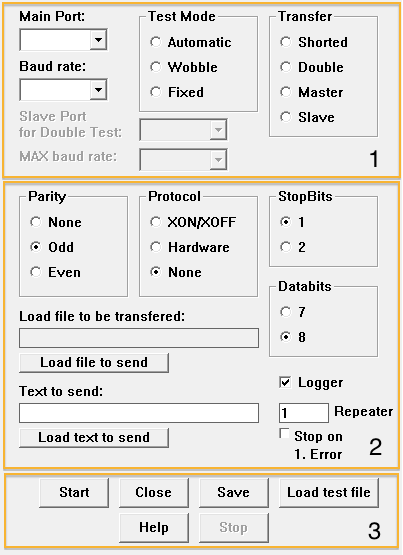
\includegraphics[scale=0.6]{gui.png}
  		  \caption{Design der Benutzeroberfläche}
  		  %\footnotesize{Quelle: www.pololu.com}
     \label{fig.3pi-m3pi-Module}
  \end{center}
\end{figure}


Die Benutzeroberfläche ist in drei Abteilungen geteilt. Die verschidene Abteilungen sind in Abbildung 5.1 zu erkennen. Genaueres zu alle Parametern wird in Kapitel ~\ref{chp:bedienungsanleitung} und  ~\ref{chp:fachlichesumfeld} erläutert. Die erste Reihe von Einstellungen hantieren die Testeinstellungen. Diese Einstellung sind:
\begin{itemize}
\item Main Port: welches COM Port soll getestet werden.
\item Baud rate: beschreibt mit welcher Baudrate der ausgewählte Port getestet werden soll.
\item Test Mode: definiert welcher Testvorgang der Benutzer haben will.
\item Transfer: legt fest, wie die Kommunikation dieses Ports stattfinden wird.
\end{itemize}


Die zwei ausgegraute Einstellungen ("`Slave Port for Double Test"' und "`MAX baud rate"') sind abhängig vor der Einstellungen in "`Test Mode"' und "`Transfer"'.\\\\


Die zweite Abteilung von Einstellungen sind die Übertragungsparameter und drei weitere Testeinstellungen. Diese Parameter sind:
\begin{itemize}
\item Parity: Paritätsüberprüfung.
\item Protocol: Übertragungsprotokoll.
\item Stopbits: Anzahl der Stopbits.
\item Databits: Anzahl der Datenbits.
\item Logger: definiert ob eine Log-Datei erstellt werden soll.
\item Repeater: Anzahl der Testwiederholungen.
\item Stop on 1. Error: bestimmt ob bei der ersten Fehlererkennung angehalten werden soll.
\item Load file to be transfered: Übertragungsdatei.
\item Text to send: Übertragungstext.\\\\
\end{itemize}


Die letzte Reihe von Elemente in der Benutzeroberfläche sind die Knöpfe. Diese führen die jeweilige Vorgange aus.
\begin{itemize}
\item Start: startet ein Test.
\item Close: schließt das Test Tool.
\item Save: speichert in eine Testdatei die Einstellungen.
\item Load test file: ladet eine Datei die im Test übertragen wird.
\item Help: zeigt ein Fenster mit Erklärungen zum Test Tool.
\item Stop: stoppt der laufende Test.\\\\
\end{itemize}


Bei drücken des Start-, Save- oder "`Load test file"'knopfes werden die Testeinstellungen an die Klasse \textit{Interpreter} weitergegeben und dort werden diese verarbeitet.


\subsection{Aufbau}

\paragraph{}
Die Klasse hinter der Benutzeroberfläche besteht aus zwei Teilen. Das erste Teil bearbeitet die Eingabe des Benutzer und der Aufbau der Oberfläche, das zweite Teil die Weitererarbeitung der Daten.\\


Das erste Teil besteht aus die Methode \textit{HandleMessage}, diese Methode ist die Fensterprozedur. Als erstes werden die Elemente, mit der Ankunft der Nachricht \textit{WM\_CREATE},des Fensters aufgebaut. Danach wird auf die Nachricht \textit{WM\_COMMAND} gewartet und jeweils reagiert. Wird zum Beispiel das Start Knopf gedrückt, bekommt die \textit{HandleMessage} die \textit{WM\_COMMAND} Nachricht mit dem Parameter \textit{ID\_BT\_START}. Das ist die Identifikationsnummer im Programm für das Start Knopf.\\
\lstset{language=C++,
				backgroundcolor=\color{white},
				%frame=single,
				tabsize=2,
				numbers=left,
				numbersep=5pt,
				%numberstyle=\color{light-gray},
				basicstyle=\ttfamily\color{black}\small,
				keywordstyle=\color{HKS51}\bfseries,
				commentstyle=\color{HKS13}\slshape,,
				identifierstyle=\color{black}}
\begin{lstlisting}	 
    case WM_CREATE:
        {
            //Create all GUI Elements
            
            //example: Start button
            _hwnd_Start = CreateWindowA("button", "Start",
				WS_CHILD | WS_VISIBLE,
				POS_X + 20, POS_Y2 + 290, 70, 30, m_hwnd, (HMENU)ID_BT_START,
				NULL, NULL);
        }
        break;
\end{lstlisting}

Wenn der Start Knopf gedrückt worden ist, fängt das zweite Teil der Klasse an. Das zweite Teil besteht aus die Weiterverarbeitung der Eingaben. Im Fall vom Start Knopf, wird als erstes einen neuen Thread aufgerufen. So kann die Benutzeroberfläche immer noch Nachrichten verarbeiten, während im Hintergrund, das Programm die Datenverarbeitung beginnt. Der gleiche Vorgang geschieht, wenn der \textit{Load test file} gedrückt wird.\\


Im Fall vom Start Knopf, ruft das Thread die Methode \textit{sendTestSettings} auf, die die Eingaben weiter gibt. Dies geschieht in dem ein Objekt der Klasse \textit{Interpreter} erzeugt wird und dessen Eigenschaften werden gesetzt.

\lstset{language=C++,
				backgroundcolor=\color{white},
				%frame=single,
				tabsize=2,
				numbers=left,
				numbersep=5pt,
				%numberstyle=\color{light-gray},
				basicstyle=\ttfamily\color{black}\small,
				keywordstyle=\color{HKS51}\bfseries,
				commentstyle=\color{HKS13}\slshape,,
				identifierstyle=\color{black}}
\begin{lstlisting}	 
	case WM_COMMAND:
	{
		//React to GUI Elements actions
		//example: Start button
		case ID_BT_START:

			//hide the elements while testing
			viewAllElements(FALSE);

			//start a new thread
			_t1 = thread(&Window::sendTestSettings, this);

			//detach the thread so it can test and main thread waits
			//for it to finish or waits for the user to press stop
			_t1.detach();
	}
    break;
\end{lstlisting}




%****************************************************************************************
\newpage
%****************************************************************************************

\section{Klasse Interpreter}
\subsection{Aufgaben}
\paragraph{}
Die Klasse \textit{Interpreter} trennt die Benutzeroberfläche von die Fachlogik des Programms. Die Benutzeroberfläche kann den Interpreter aufrufen und hat Zugriff auf die \textit{public} Methoden der Klasse. Der Interpreter kann nicht auf Elemente oder Methoden der Klasse \textit{Window} zugreiffen. Durch diese Trennung kann den Benutzer nie die auf die Fachlogik zugreifen, nur über die Möglichkeiten die der Programmierer anbietet.\\

Eine Aufgabe des Interpreters ist die Überprüfung der Eingaben des Benutzers bevor die Tests beginnen. Durch "`setter"' Methoden werden die Eingabeparameter der GUI in lokalen Variablen gespeichert.\\

\lstset{language=C++,
				backgroundcolor=\color{white},
				%frame=single,
				tabsize=2,
				numbers=left,
				numbersep=5pt,
				%numberstyle=\color{light-gray},
				basicstyle=\ttfamily\color{black}\small,
				keywordstyle=\color{HKS51}\bfseries,
				commentstyle=\color{HKS13}\slshape,,
				identifierstyle=\color{black}}
\begin{lstlisting}	 
void Interpreter::setTransfer(int iTransfer)
{
	this->_iTransfer = iTransfer;
}
\end{lstlisting}

Danach werden die lokalen Variablen auf Fehleingaben geprüft. Sind Fehler erkannt worden, werden diese dem Benutzer bekannt gemacht und alle Parameter in der Klasse werden auf ein Standardwert zurückgesetzt. Sind keine Fehleingaben erkannt, werden die Werte der Variablen in einer Datenstruktur gespeichert. Mehr zu dieser Struktur erfahren sie im Kapitel ~\ref{TestStruct}. Folgende Codezeilen stellen dar, wie so ein Vorgang aussieht. Hier wird nach dem Übertragungsmodus abgefragt.

\lstset{language=C++,
				backgroundcolor=\color{white},
				%frame=single,
				tabsize=2,
				numbers=left,
				numbersep=5pt,
				%numberstyle=\color{light-gray},
				basicstyle=\ttfamily\color{black}\small,
				keywordstyle=\color{HKS51}\bfseries,
				commentstyle=\color{HKS13}\slshape,,
				identifierstyle=\color{black}}
\begin{lstlisting}	 
if (_iTransfer == DEFAULT_VALUE)
{
	MessageBoxA(NULL,"Please select a transfer mode",
							WINDOW_TITLE, MB_OK | MB_ICONERROR);
	setDefaultValues();
}
else
{
	//save the transfer mode
	_testManager->testStruct.iTransfer = _iTransfer;
}
\end{lstlisting}

Die Werte in den Variablen müssen überprüft werden, um Fehler zu vermeiden. Da die Werte nicht nur aus Einstellungen in der Benutzeroberfläche stammen, sondern auch aus eine Testkonfigurationsdatei, können falsche Eingabe vorhanden sein.\\

Außer die Überprüfung der Eingabeparameter und setzen der lokalen Variablen, gibt diese Klasse die Testeinstellungen an die anderen Klassen weiter. Hier trennt sich das Programm in zwei Pfade. Das erste Pfad gibt die Datenstruktur an die Klasse \textit{TestManager} weiter. Der zweite Pfad speichert oder liest eine Testkonfigurationsdatei. Im Fall, dass eine Testkonfigurationsdatei gelesen werden soll, wird als erstes die Klasse \textit{IniFileHandler} aufgerufen und danach die Klasse \textit{TestManager}, damit ein Test mit den gelesenen Einstellungen gestartet wird. Sollen die Eingabeparameter der Benutzeroberfläche in einer Testkonfigurationsdatei gespeichert werden, werden die überprüfte Eingabeparameter in einer vom Benutzer angegebene Datei gespeichert. Dafür wird auch die Klasse \textit{IniFileHandler} aufgerufen.\\

Da die Klasse \textit{Interpreter} die Schnittstelle für die Kommunikation zwischen Fachlogik und Benutzer ist, wird auch durch diese Klasse die Meldung gegeben, ein Test zu anhalten. Durch das Klicken des Button "`Stop"' in der Benutzeroberfläche wird eine boolische Variable weiter an die Testlogik gegeben. Diese Variable wird vor jedem Testschleife abgefragt, ist sie gesetzt, dann wird das Testen angehalten.\\

Die Klasse hat ein Objekt der Klasse \textit{Com}, um in der Benutzeroberfläche die im System zur Verfügung stehende COM Ports aufgelistet werden können. Durch die Trennung der GUI mit der Fachlogik, darf die \textit{Window} Klasse kein Objekt der Klasse \textit{Com} haben.\\



%****************************************************************************************
\newpage
%****************************************************************************************

\section{Struktur TestStruct}\label{TestStruct}
\subsection{Definition}
\paragraph{}
Ein \textit{struct} oder Struktur dient dazu, mehrere logische zusammenhängende Variablen verschiedener Datentypen zusammenzufassen. In \textit{C} beinhalten Strukturen nur Variablen, in \textit{C++} wurden die Strukturen erweitert und dürfen auch Funktionen beinhalten. Dadurch ist der Unterschied zu einer Klasse nur die Zugriffsrechte auf die Eigenschaften. In einer Struktur sind die Zugriffsrechte auf Elemente mit  \textit{public} definiert, in einer Klasse mit \textit{private} \footnote{Visual C++ 2010}. Da ich nur Variablen benötigte, und keine Methoden, habe ich mich für eine Struktur entschieden.


\subsection{Aufbau}
\paragraph{}
Die Datenstruktur fasst alle Eigenschaften für einem Test zusammen. Die \textit{TestStruct} beinhaltelt folgende Variablen und wird so definiert:\\
\lstset{language=C++,
				backgroundcolor=\color{white},
				%frame=single,
				tabsize=2,
				numbers=left,
				numbersep=5pt,
				%numberstyle=\color{light-gray},
				basicstyle=\ttfamily\color{black}\small,
				keywordstyle=\color{HKS51}\bfseries,
				commentstyle=\color{HKS13}\slshape,,
				identifierstyle=\color{black}}
\begin{lstlisting}	 
struct TestStruct
{
	string sMasterPort;
	string sSlavePort;
	string sTextToTransfer;
	string sFilePath;
	int iTransfer;
	int iBaud;
	int iBaudrateMax;
	int iTestMode;
	int iParity;
	int iProtocol;
	int iStopbits;
	int iDatabits;
	int iTransTextMode;
	int iRepeater;
	bool bLoggerState;
	bool bStopOnError;
	vector<string> svBaudrates;
}
\end{lstlisting}

Jeder dieser Variablen stellt ein Wert dar, für eine Einstellung in der Benutzeroberfläche. Für eine genauere Erläuterung der Variablen und dessen Werte, bitte siehe Kapitel \ref{chp:bedienungsanleitung} und ~\ref{IniFileHandler}.

%****************************************************************************************
\newpage
%****************************************************************************************


\section{Klasse Com}
\subsection{Aufbau}
\paragraph{}
Die Klasse \textit{Com} fasst alles um die Verwaltung eines COM Ports um. Um aus einem COM Port lesen und schreiben zu können, müssen zuerst die Eigenschaften des jeweiligen Ports gesetzt werden. Alle Ports in einem System werden beim Systemstart mit einer Standardkonfiguration konfiguriert. Will der Benutzer Peripherieelemente an einem COM Port anschließen, die nicht die gleiche Konfiguration besitzt wie die  im System vordefiniert, muss die Konfiguration des Ports angepasst werden. Dafür muss ein COM Port zuerst geöffnet werden, danach kann die Konfiguration geändert werden. Wenn diese beide Schritte erfolgreich abgelaufen sind, können aus dem COM Port Informationen gesendet und empfangt werden. Als letzter Schritt ist sehr wichtig der benutze COM Port wieder zu schließen. Somit steht der COM Port wieder andere Applikationen und das System zur Verfügung.\\

\subsection{Aufgaben}
\paragraph{}
Das Öffnen eines Ports benutzt die gleiche Systemfunktion wie um eine Datei zu erzeugen. Die Funktion \textit{CreateFile} gibt ein Handle auf das gewünschte Port. Durch dieses Handle wir der jeweilige Port für andere Operationen identifiziert.

\lstset{language=C++,
				backgroundcolor=\color{white},
				%frame=single,
				tabsize=2,
				numbers=left,
				numbersep=5pt,
				%numberstyle=\color{light-gray},
				basicstyle=\ttfamily\color{black}\small,
				keywordstyle=\color{HKS51}\bfseries,
				commentstyle=\color{HKS13}\slshape,,
				identifierstyle=\color{black}}
\begin{lstlisting}	 
hCom = CreateFile(portNumber.c_str(),  
            GENERIC_READ|GENERIC_WRITE,
            0, 
            NULL,
            OPEN_EXISTING, 
            FILE_FLAG_OVERLAPPED,
            NULL); 

\end{lstlisting}

Das erste Parameter der Funktion ist der Name des gewünschtes Ports. Besitzt der COM Port einen Wert von eins bis neun wird ein Wert wie "`COM5"' gesetzt. Ist der Wert des Ports größer neuen und maximal 256 muss der erste Parameter folgendermaßen gesetzt werden: "`\textbackslash\textbackslash.\textbackslash COM255"'. Der zweite Parameter beschreibt die Zugriffsrechte auf der COM Port. Da wir Informationen senden und empfangen möchten, braucht das Programm Lese- und Schreibrechte. Sehr wichtig ist der fünfte Parameter. Dieser beschreibt das nur existierende COM Ports geöffnet werden sollen. Da die Funktion auch Dateien erzeugen kann, sind diese nicht vorhanden sind, werden sie kreiert. Im Fall von COM Ports sollen keine erzeugt werden, sondern die als Hardware vorhandene Ports öffnen. \textit{FILE\_FLAG\_OVERLAPPED} setzt die Eingenschaft, dass der COM Port im asynchron Modus geöffnet werden soll.\\

Damit den Benutzer, in der Benutzeroberfläche, nicht vorhandene COM Ports angeboten werden, wird bei der Aufbau der GUI alle zur Verfügung stehende COM Ports aufgelistet. Dafür wird in einer Schleife versucht alle COM Ports zwischen Null bis 256 zu öffnen, die Ports die einen nicht ungültigen Handle zurück geben werden aufgelistet.\\


Wenn ein COM Port nicht erfolgreich geöffnet werden konnte, gibt die \textit{CreateFile} Funktion ein nicht valides Handle zurück. Wird ein Port erfolgreich geöffnet, können die Eigenschaften des Ports bearbeitet werden. Wie in Kapitel ~\ref{COMWINAPI} erklärt, werden die Eigenschaften des Ports durch verschiedene Strukturen gesetzt.\\

Für jeden Test kann der Benutzer die Baudrate einstellen. In der Benutzeroberfläche, wird in Form einer Liste in einem Combo Box, die unterstützten Baudrate aufgelistet. Um die Baudraten zu ermitteln muss zuerst die Struktur \textit{COMMPROP} geladen werden. In der Variable \textit{dwSettableBaud} sind als Bitmaske die unterstützten Baudraten gespeichert. Das Algorithmus dafür sieht so aus:
\lstset{language=C++,
				backgroundcolor=\color{white},
				%frame=single,
				tabsize=2,
				numbers=left,
				numbersep=5pt,
				%numberstyle=\color{light-gray},
				basicstyle=\ttfamily\color{black}\small,
				keywordstyle=\color{HKS51}\bfseries,
				commentstyle=\color{HKS13}\slshape,,
				identifierstyle=\color{black}}
\begin{lstlisting}
	//Lade die COMMPROP Stuktur des geöffneten Ports	 
	GetCommProperties(hCom, &commProp);
 
 	//Bitmaske mit den unterstützten Baudraten
	bitset<32> bitMask ((int)commProp.dwSettableBaud);
	
	//ignoriere die letzte 4 bits
	for( int i = 0; i < 28; i++)
	{
		//falls das Bit gesetzt ist
		if (bitMask.test(i) == true)
		{
			//dann wird die Baudrate unterstützt
			vBaud.push_back(saDefaultBaudrates[i]);
		}
	}
\end{lstlisting}

In der Schleife wird geprüft ob der jeweilige Bit an der Stelle "`i"' eine Eins oder Null ist. Falls es eine Eins ist, dann wird die Baudrate im Array an der Stelle "`i"' in eine Vektor gespeichert. In diesem Vektor werden alle Baudraten gespeichert, die vom angegebene Port unterstützt werden. Der Vektor gehört zur \textit{Com} Klasse und wird durch das ganze Programm benutzt.\\



 KONSTRUKTOREN
 
 AUFLISTUNG DER PORTS
%****************************************************************************************
\newpage
%****************************************************************************************


\section{Klasse PortCommunications}
\paragraph{}

\subsection{}


%****************************************************************************************
\newpage
%****************************************************************************************


\section{Klasse TestManager}
\paragraph{}

\subsection{}

%****************************************************************************************
\newpage
%****************************************************************************************


\section{Klasse FixedTest}
\paragraph{}

\subsection{}

%****************************************************************************************
\newpage
%****************************************************************************************


\section{Klasse IniFileHandler}\label{IniFileHandler}
\paragraph{}
erklaren aller parameter und mögliche werte
\subsection{}

%****************************************************************************************
\newpage
%****************************************************************************************


\section{Klasse Logger}
\paragraph{}

\subsection{}

%****************************************************************************************
\newpage
%****************************************************************************************


\section{Klasse Tools}
\paragraph{}

\subsection{}

%****************************************************************************************
\newpage
%****************************************************************************************


\section{Klasse TransferFileHandler}
\paragraph{}

\subsection{}